%!TEX root = ../presentation.tex

\begin{frame}{Examples}
    \textbf{Example: L-shaped panel test}
\begin{minipage}{1.0\textwidth}
\begin{minipage}{0.5\textwidth}
    \begin{itemize}
        \item L-shaped concrete slab, subjected to mode I failure
        \item Displacement controlled experiment
        \item Crack emanating from the reentrant corner
    \end{itemize}
\end{minipage}%
\hfill{}%
\begin{minipage}{0.4\textwidth}
    \centering
    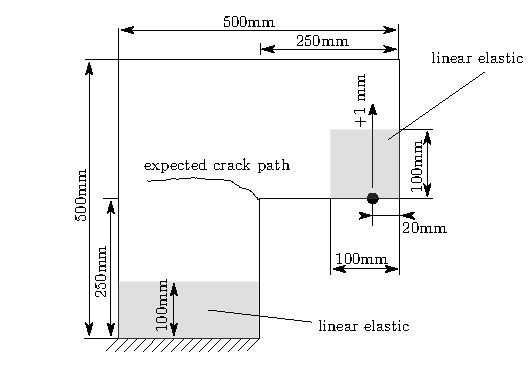
\includegraphics[height=3.0cm]{\slidedir/winkler_setup.pdf}%
\end{minipage}
\end{minipage}

\vfill

\begin{minipage}{1.0\textwidth}
    \begin{figure}[htpb]
        \centering
        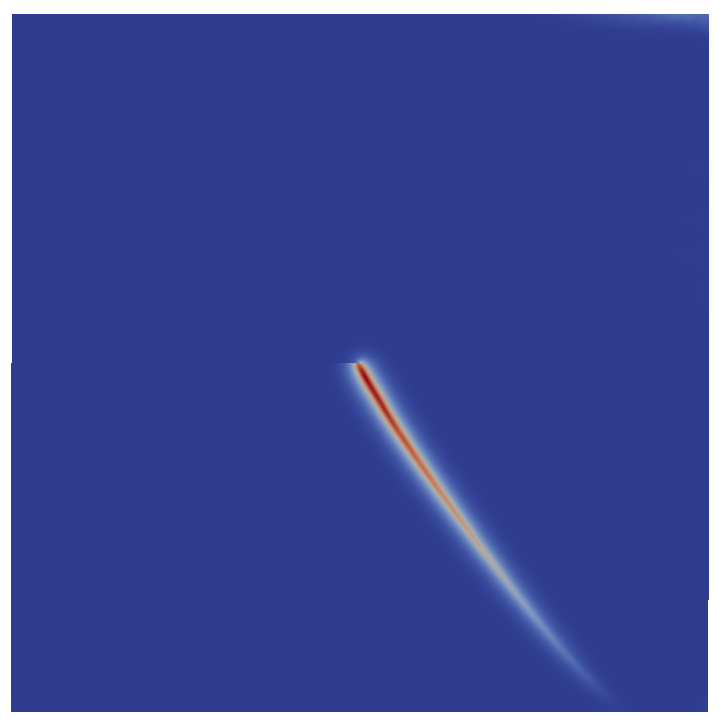
\includegraphics[width=0.3\linewidth]{\slidedir/ge_rankine_nldamage_cropped.png}
        \caption{Predicted crack paths: Gradient-enhanced Rankine (left), ....}%
        \label{fig:name}
    \end{figure}
\end{minipage}
\end{frame}
